
\documentclass[english,final,t]{beamer}

\usepackage[orientation=landscape,size=a0, scale=1.35]{beamerposter}
\usepackage[T1]{fontenc}
\usepackage[latin9]{inputenc}
\usepackage{lmodern}
\usepackage{babel}            
\usefonttheme{serif}          
\usepackage[scaled]{beramono}  
\usepackage{helvet}        
\usepackage{cleveref}   
\renewcommand{\familydefault}{\sfdefault}

\mode<presentation>
{\usetheme{Tikhonov}}
\setbeamercovered{transparent}

\usepackage[mathscr]{euscript}
\usepackage{amsthm}       
\usepackage{ragged2e}                             
\usepackage{amssymb}                                    
\usepackage{amsmath}                                    
\usepackage{graphicx}                                   
\usepackage{enumerate}                                  
\usepackage{pdflscape}                                            

\title{\huge Parameter symmetry in perturbed GUE corners process}
\author[Tikhonov]{Mikhail Tikhonov}
\institute[University of Virginia, IITP]{Department of Mathematics, University of Virginia and Institute for Information Transmission Problems}
\date{\today}

\newtheorem{proposition}{Proposition}[section]
\newtheorem{question}{Open problem}
\begin{document}
\begin{frame}{}
    \begin{columns}[t]
        \begin{column}{.26\linewidth}

            \begin{block}{Introduction}
\justifying
This poster is based on joint work with L. Petrov \cite{PetrovTikhonov2020}.
We present a new symmetry
of the distribution of the \emph{perturbed GUE
ensemble}. By this we mean the random matrix ensemble
of the form $H=G+\mathrm{diag}(a_1,\ldots,a_N)$, where $G$ is an $N\times N$
GUE random matrix, to which we add a fixed diagonal matrix. 


Together with the eigenvalues $\lambda^N=(\lambda^N_N\le \ldots\le\lambda^N_1 )$,
$\lambda^N_i\in \mathbb{R}$,
of the full matrix $H=[h_{ij}]_{i,j=1}^{N}$, 
one can also
consider its
\emph{corners process},
cf. \cite{johansson2006eigenvalues}.
that is, the interlacing collection of eigenvalues
of the principal corners
$[h_{ij}]_{i,j=1}^{k}$ of $H$ for all $k=1,2,\ldots,N $.
The distribution of the corners process of $H$ is 
\emph{not symmetric} in the parameters $a_i$.

\begin{figure}[htpb]
	\centering
	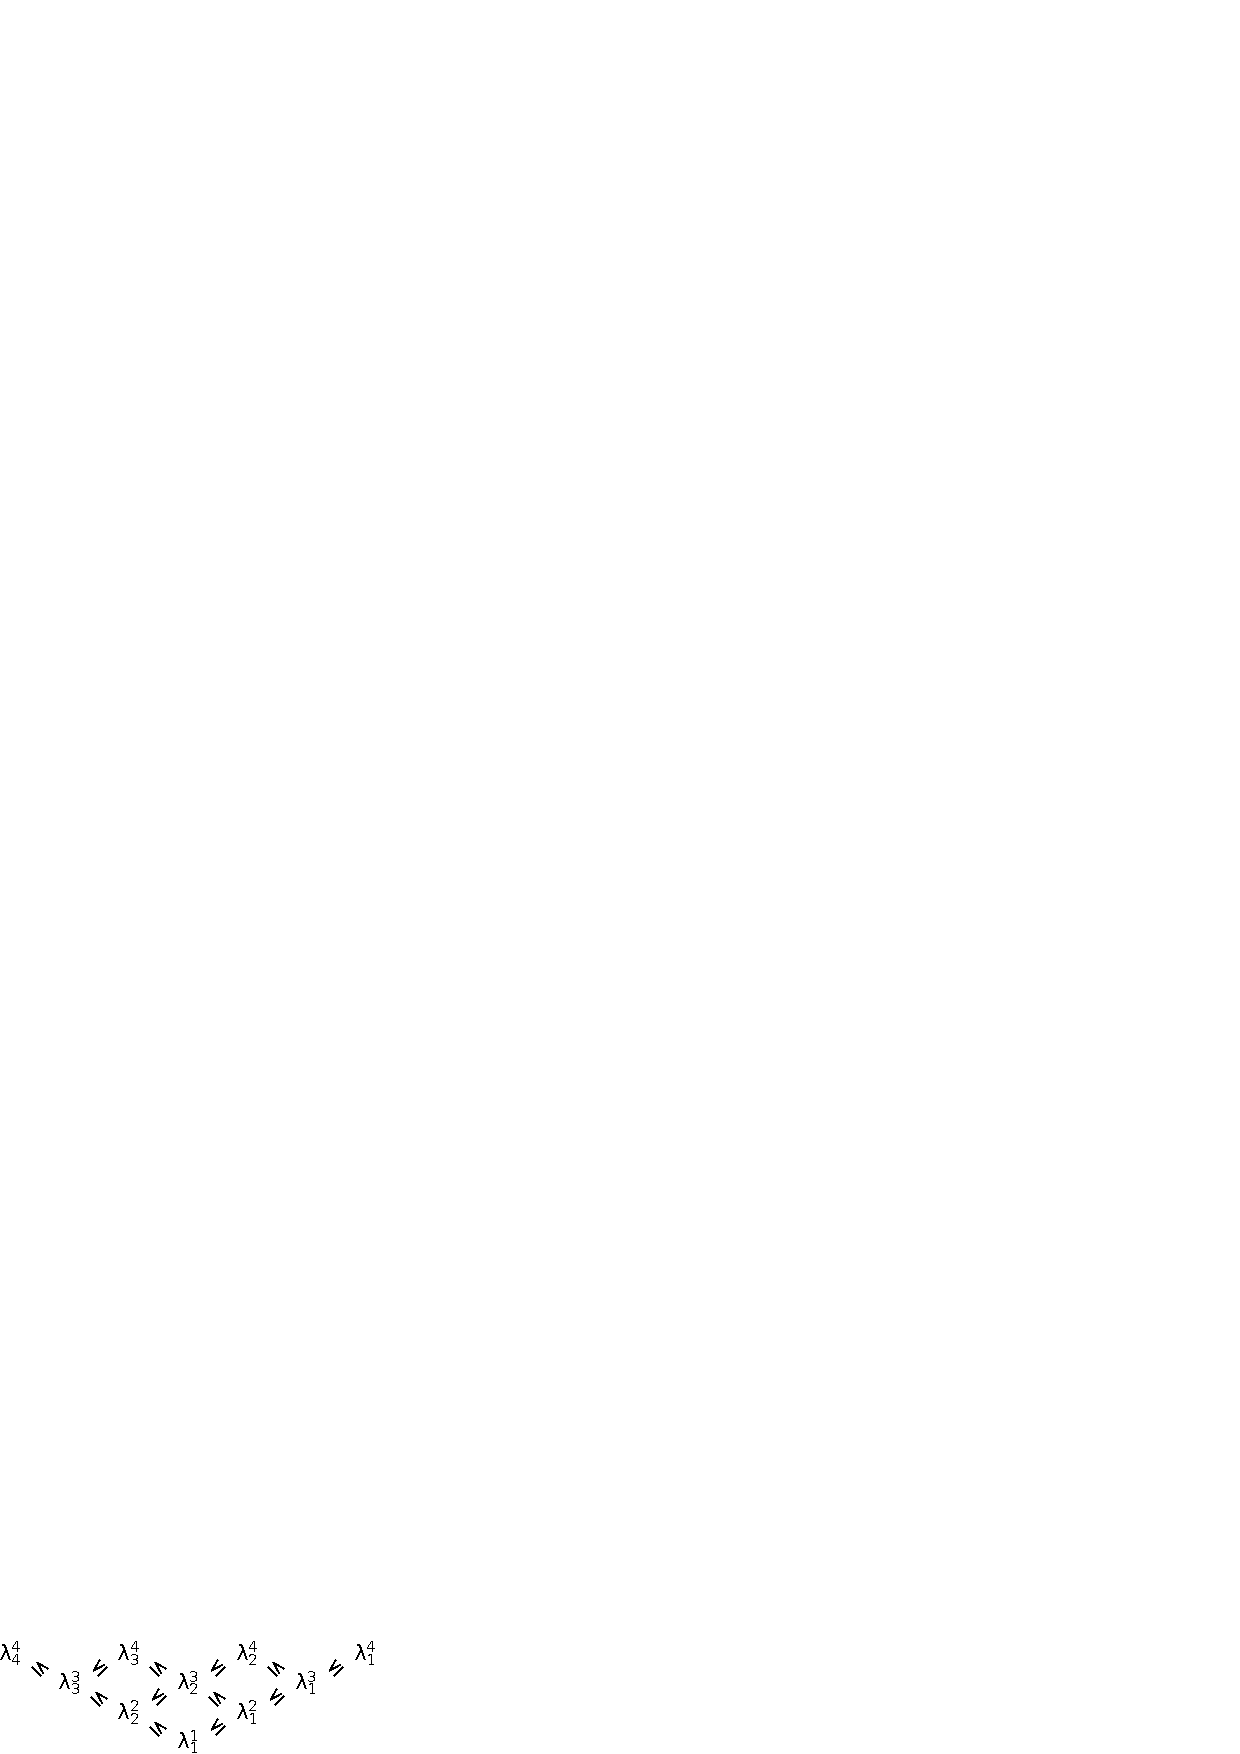
\includegraphics[width=.55\textwidth]{fig_interlace.pdf}
	\caption{Interlacing array of eigenvalues
	of all principal corners of a $4\times 4$ matrix.}
	\label{fig:interlace}
\end{figure}

We show that each nearest neighbour transposition
$a_k\leftrightarrow a_{k+1}$, $k=1,\ldots,N-1 $, of the parameters
is equivalent in distribution to a 
rather simple \emph{Markov swap operator}
$\mathscr{S}^{a_k-a_{k+1}}_k$. 
This swap operator
randomly changes the entries $\lambda^k_i$
on the $k$-th level of the array given the 
two adjacent levels $\lambda^{k-1},\lambda^{k+1}$,
while leaving all other entries intact.
If $a_k>a_{k+1}$, 
$\mathscr{S}^{a_k-a_{k+1}}_k$
is realized as an independent collection of instantaneous
exponential type jumps of each $\lambda^k_i$
to the left:
\begin{equation*}
    	\lambda^{k}_i\mapsto \nu^k_i:=
	\lambda^{k+1}_{i+1}\vee \lambda^{k-1}_{i}
	+
	\mathscr{E}_{a_k-a_{k+1}}^i\wedge
	\bigl(
		\lambda^k_i-
		\lambda^{k+1}_{i+1}\vee \lambda^{k-1}_{i}
	\bigr),
\end{equation*}
where $\mathscr{E}_{a_k-a_{k+1}}^{i}$'s are independent exponential random variables
with parameter $a_k-a_{k+1}$ (and mean $1 / (a_k-a_{k+1})$).
            \end{block}
            \begin{figure}[htpb]
                \centering
                \includegraphics[width=.9\textwidth]{eigenvalues_jump.pdf}
                \label{fig:jump}
            \end{figure}
\begin{theorem}
    \label{thm:main_swap}
    Assume that $a_k\ne a_{k+1}$. Then the action of the Markov operator
    $\mathscr{S}^{a_k-a_{k+1}}_k$ (with left jumps for $a_k>a_{k+1}$, and right jumps otherwise)
    turns the corners distribution of $G+\mathrm{diag}(a_1,\ldots,a_k,a_{k+1},\ldots,a_N )$
    into the one of $G+\mathrm{diag}(a_1,\ldots,a_{k+1},a_{k},\ldots,a_N )$,
    where $G$ is the $N\times N$ GUE random matrix.
\end{theorem} 

\end{column}
\begin{column}{.26\linewidth}
    \begin{theorem}
        \label{thm:main_theorem_shift}
        The action of a sequence of left exponential jumps 
        (where the parameter at level $k$ is taken to be $k\alpha$), from level $1$
        up to infinity, is equivalent in distribution 
        to shifting all the 
        elements of the interlacing array by $\alpha$ to the left.
    \end{theorem}  

\begin{block}{Brownian Motions}
\justifying
    

Fix a perturbation sequence $\mathbf{a}=\{a_i \}_{i\in \mathbb{Z}_{\ge1}}$.
Consider a family of interacting Brownian motions 
$B^k_j$, $1\le j\le k<\infty$, such that:
\begin{itemize}
	\item All processes start from zero.
	\item The processes $B^k_j$, $j=1,\ldots,k $
		have the same drift $a_k$.
	\item The evolution of each $B^k_j$
		does not depend on any of the $B^l_i$'s with $l>i$.
	\item The processes interact only through their local times.
		That is, when the processes are sufficiently far apart,
		each $B^k_j$ behaves as an independent Brownian motion 
		with drift $a_k$.
	\item Each $B^k_j$ belongs to the segment
		$[B^{k-1}_j,B^{k-1}_{j-1}]$
		and reflects off 
		both 
		$B^{k-1}_j$ and $B^{k-1}_{j-1}$.
		Therefore, at each time $t$, the 
		random variables
		$\{B^k_j(t)\}_{1\le j\le k<\infty}$ almost surely form
		an interlacing array as in \Cref{fig:interlace}.
\end{itemize}
\end{block}
\begin{figure}[bm]
	\centering
	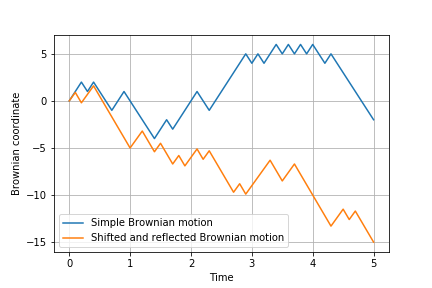
\includegraphics[width=.9\textwidth]{reflected_bm.png}
	\label{fig:bm}
\end{figure}
\begin{proposition}[Theorem 2 from \cite{ferrari2014perturbedGUE}]
	\label{prop:connection_to_reflected_BM}
	At each fixed time moment $t\in \mathbb{R}_{\ge0}$, we have equality
	of joint distributions of two infinite interlacing arrays:
	\begin{equation*}
		\{B^k_j(t)\}_{1\le j\le k<\infty}
		\stackrel{d}{=}
		\{\lambda^k_j\}_{1\le j\le k<\infty},
	\end{equation*}
	where the right-hand side is the perturbed GUE
	corners process with the same time parameter $t$
	and perturbation sequence $\mathbf{a}$.
\end{proposition}

        \end{column}

        \begin{column}{.26\linewidth}
            \begin{proposition}
                \label{prop:elementary_swap}
                Take real numbers $c<d$ and $\alpha>0$. 
                Let $X$ be distributed as $E_\alpha(c,d)$,
                and $\mathscr{E}_\alpha\in(0,+\infty)$ be an independent usual
                exponential random variable with parameter $\alpha$
                (i.e., with density $\alpha e^{-\alpha y}$, $y>0$). Then
                the random variable
                \begin{equation}
                    \label{eq:Y_as_function_of_X_elementary_swap}
                    Y:=c+\mathcal{E}_\alpha\wedge(X-c)
                \end{equation}
                is distributed as $E_{-\alpha}(c,d)$.
            \end{proposition}
            \begin{question}
                Is it possible to construct a Markov operator 
                on whole trajectories $t\mapsto \{X_k(t) \}_{k\in \mathbb{Z}_{\ge1}}$
                which is equivalent in distribution to a shift of 
                reflected Brownian motions as stochastic processes?
            \end{question}
            \begin{question}
                Do there exist well-defined $\alpha\searrow0$ limits of the Markov operators acting 
                on the GUE corners process perturbed by an arithmetic progression $a_i=-(i-1)\alpha$
                or on the reflected drifted Brownian motions? 
                These hypothetical limits should act on (much more studied)
                unperturbed GUE corners process and driftless reflected Brownian motions.
            \end{question}
            \begin{block}{References}
                \bibliographystyle{unsrt}
                \bibliography{bib}
            \end{block}
        \end{column}
    \end{columns}
\end{frame}
\nocite{warren2005dyson}


\end{document}